
Modulul de acces la date este interfate web prin intermediul careia vizitatorii site-ului vor putea sa vada seturile de date disponibile in arhiva RODA si sa obtina date statistice suplimentare despre variabilele fiecarui studiu in parte. 

\section{Tehnologie}

Modulul e acces la date este construit cu ajutorul acelorasi tehnologii ca si modulul de administrare prezentat in capitolul anterior, sistemul de biblioteci Javascript ExtJS care comunica cu serverul folosind JSON. 


\section{Arhitectura}

Ca orice aplicatie ExtJS, toate componentene modulului de acces la date se inscriu intr-un container principal care, spre deosebire de interfata de administrare unde ocupa intreaga fereastra a browserului (tip viewport), aici este un container definit intr-o pagina HTML care are si alte elemente. In continuare se poate vedea o versiune simplificata a paginii in care este inclusa aplicatia de acces la date. Se observa in interiorul div-ului cu id "content" un div al carui id se numeste "dbcontainer". 
In acest div cu id-ul dbcontainer se va incarca aplicatia de acces la date.

\begin{lstlisting}[language=HTML]
<body>
		<div id="pgheader">
		</div>
		<div id="content">
			<div id="dbcontainer" style="width:80%; height:100%; padding: 0; margin-left:auto; margin-right:auto;"></div>
	 	</div>
	<div id="pgfooter"></div>
</body>
\end{lstlisting}

In continuare se poate observa functia care este responsabila de initializarea databrowserului. Pentru a putea asigura faptul ca aplicatia va ocupa intregul container se foloseste un plugin suplimentar numit "fittoparent", a carei declaratie se poate observa in functie, imediat dupa specificarea id-ului containerului parinte. 


\begin{lstlisting}[language=json]
    init : function() {  	
    	console.log('init');
    	Ext.Ajax.timeout = 200000; 
	    Ext.override(Ext.form.Basic, {     timeout: Ext.Ajax.timeout / 1000 });
	    Ext.override(Ext.data.proxy.Server, {     timeout: Ext.Ajax.timeout });
	    Ext.override(Ext.data.Connection, {     timeout: Ext.Ajax.timeout });
	    Ext.create('databrowser.view.DataBrowserPanel',{
	         renderTo: 'dbcontainer',
	         plugins : ['fittoparent'],
	     })
	  },
\end{lstlisting}

Tot in functia de initializare se poate observa numele clasei care se initializeaza si care reprezinta principala clasa a modulului, : 'databrowser.view.DataBrowserPanel'. Aceasta este o extensia a clasei 'Ext.panel.Panel' care contine doua regiuni, una mai ingusta in partea stanga in care se vor incarca alte componente si una mai lata in partea dreapta in care se vor incarca alte componente. Efectul incarcarii componentului principal se poate vedea in figura urmatoare, unde este afisat doar acesta, fara continut. 

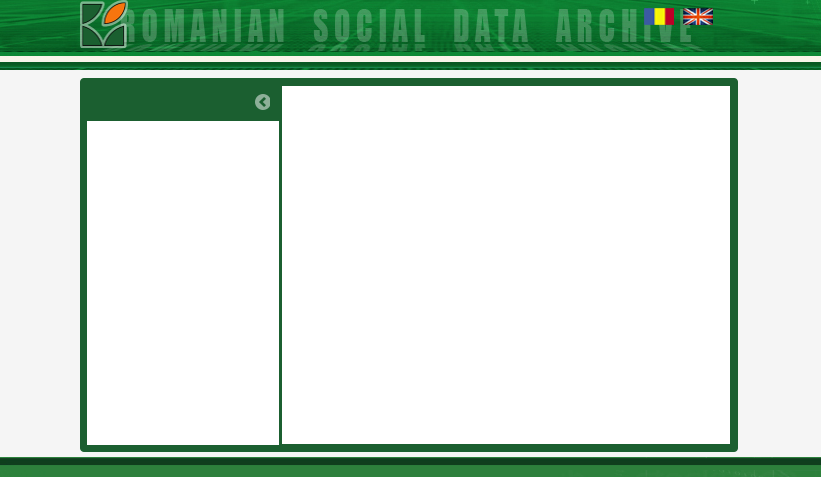
\includegraphics[width=10cm]{img/db-empty}

In figura se observa cele doua regiuni descrise. Panoul este divizat in doua subpanouri utilizand un anumit tip de layout (numit "border") care permite acestor doua panouri sa  fie redimensionate de catre operatori prin drag-and-drop. De asemenea, panoul stang poate fi minimizat prin click pe sageata de la partea superioara a acestuia. 

In fiecare panou al clasei 'databrowser.view.DataBrowserPanel' se incarca cate un component diferit, dupa cum urmeaza: 

In zona din partea stanga se incarca o clasa numita: 'databrowser.view.Browser' care contine mai multe componente, fiecare dintre ele fiind conceput astfel incar sa permita gruparea studiilor in functie de un anumit criteriu: fie dupa catalog, fie dupa anul producerii, fie dupa cuvintele cheie. Componentele sunt extensii ale componentului de 'Ext.tree.Panel' 

Selectia in functie de cataloage se poate vedea in figura urmatoare:


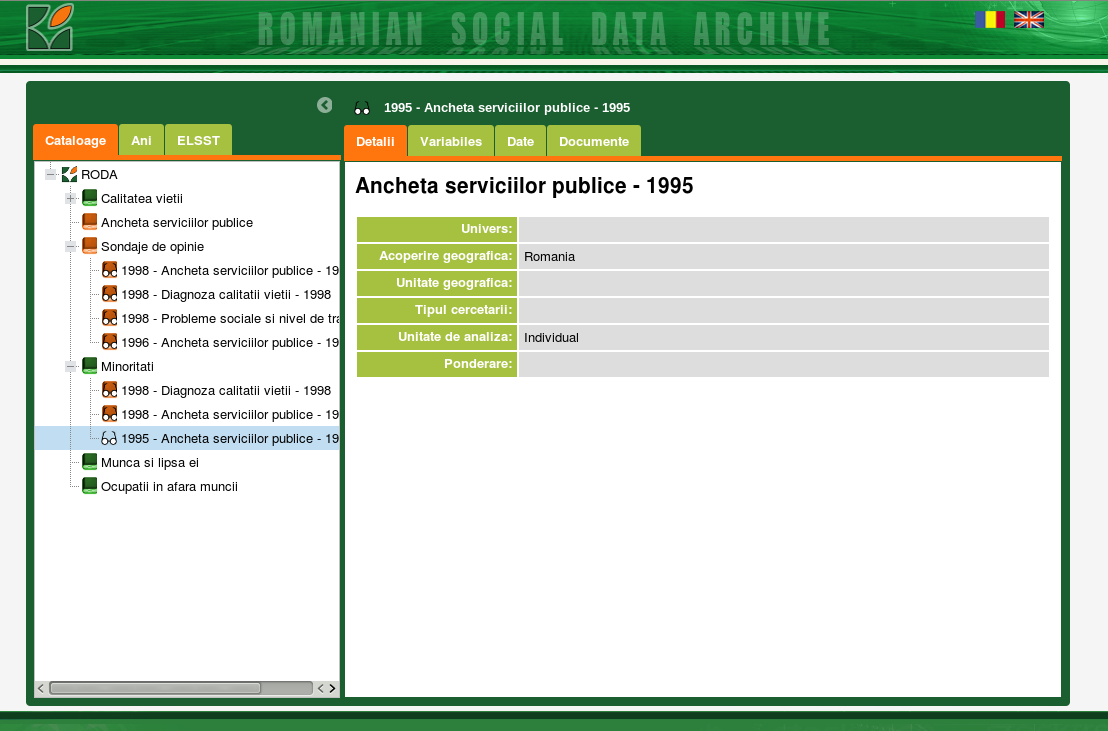
\includegraphics[width=16cm]{img/db-catalog}


\section{Afisare si comunicare}


Datele afisate in lista de cataloage sunt obtinute de la server in format JSON si arata dupa cum urmeaza


\begin{lstlisting}[language=json]
{
    "data": [
        {
            "name": "RODA",
            "type": "M",
            "data": [
                {
                    "data": [
                        {
                            "an": 1998,
                            "description": null,
                            "geographicUnit": null,
                            "indice": "42",
                            "leaf": true,
                            "name": "Reteaua de observare sociala privind problemele populatiei de rromi - 1998",
                            "researchInstrument": null,
                            "seriesId": null,
                            "type": "St",
                            "weighting": null
                        },
                        {
                            "an": 1998,
                            "description": null,
                            "geographicUnit": "a) regiuni; b)judete; c) localitati",
                            "indice": "41",
                            "leaf": true,
                            "name": "Probleme sociale si nivel de trai - 1998",
                            "researchInstrument": "Structurat",
                            "seriesId": 4,
                            "type": "Sts",
                            "weighting": null
                        },
                        {
                            "data": null,
                            "indice": "2",
                            "leaf": true,
                            "name": "Diagnoza calitatii vietii",
                            "type": "C"
                        }
                    ],
                    "indice": "1",
                    "leaf": false,
                    "name": "Calitatea vietii",
                    "type": "C"
                },
            ]
        }
    ]
}
\end{lstlisting}

Selectia studiilor in functie de ani este disponibila in subpanoul "Ani" care se poate vedea in figura urmatoare

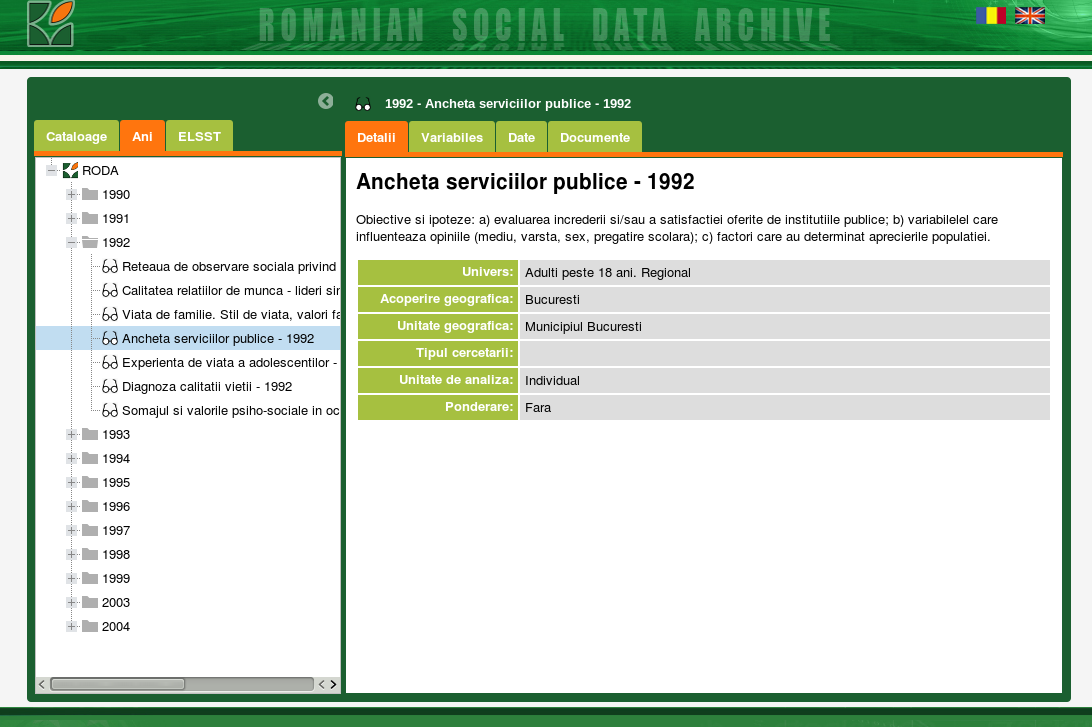
\includegraphics[width=16cm]{img/db-year}

\begin{lstlisting}[language=json]
{
    "data": [
        {
            "name": "RODA",
            "type": "M",
            "data": [
                {
                    "data": [
                        {
                            "an": 1990,
                            "description": "Cercetarea este un demers sistematic de analiza a ...",
                            "geographicUnit": "Localitatea: sat, oras",
                            "indice": "38",
                            "leaf": true,
                            "name": "Diagnoza calitatii vietii - 1990",
                            "researchInstrument": "Chestionar standardizat cu scale de tip Likert pentru perceptii, evaluare, satisfactie.",
                            "seriesId": null,
                            "type": "St",
                            "weighting": "Fara"
                        }
                    ],
                    "name": "1990",
                    "type": "Y",
                    "year": 1990
                },
                {
                    "data": [
                        {
                            "an": 1991,
                            "description": "Lucrarea a urmarit sa faca o comparatie intre calitatea ...",
                            "geographicUnit": "(a) Orase; (b) Judete; (c) Sectii de votare",
                            "indice": "36",
                            "leaf": true,
                            "name": "Calitatea vietii urbane in perioada de tranzitie. Comparativ Romania-Polonia - 1991",
                            "researchInstrument": "Structurat; chestionar cu intrebari inchise si deschise",
                            "seriesId": null,
                            "type": "St",
                            "weighting": "Nu s-au folosit ponderari"
                        },
                        {
                            "an": 1991,
                            "description": "Ipoteze si obiective Cunoasterea dimensiunilor saraciei pe ansamblu...",
                            "geographicUnit": "(a) Regiuni; (b) Judete; (c) Localitati",
                            "indice": "37",
                            "leaf": true,
                            "name": "Nivel de trai. Saracie - 1991",
                            "researchInstrument": "Structurat; chestionar cu intrebari inchise si deschise",
                            "seriesId": null,
                            "type": "St",
                            "weighting": "Nu s-au folosit ponderari"
                        }
                    ],
                    "name": "1991",
                    "type": "Y",
                    "year": 1991
                },
            ]
        }
    ]
}
\end{lstlisting}

Indiferent de modulul care se foloseste in sectiunea din partea stanga a modulului, in partea dreapta se afiseaza fie un catalog, fie o serie, fie un studiu. Studiul poate fi studiu de sine statator sau poate fi membru al unei serii. 

In cazul in care se selecteaza un studiu, panoul va incarca componentul care afiseaza detaliile unui studiu, elementele descriptive generale si lista de variabile. Lista de variabile permite accesul direct la motorul statistic. Exista doua categori de analize disponibile, analize univariate (cele care se executa la selectia unei singure variabile) sau analize bivariate (cele disponibile la selectia adoua variabile). 

In figura urmatoare se poate vedea rezultatul unei analize pe o singura variabila:

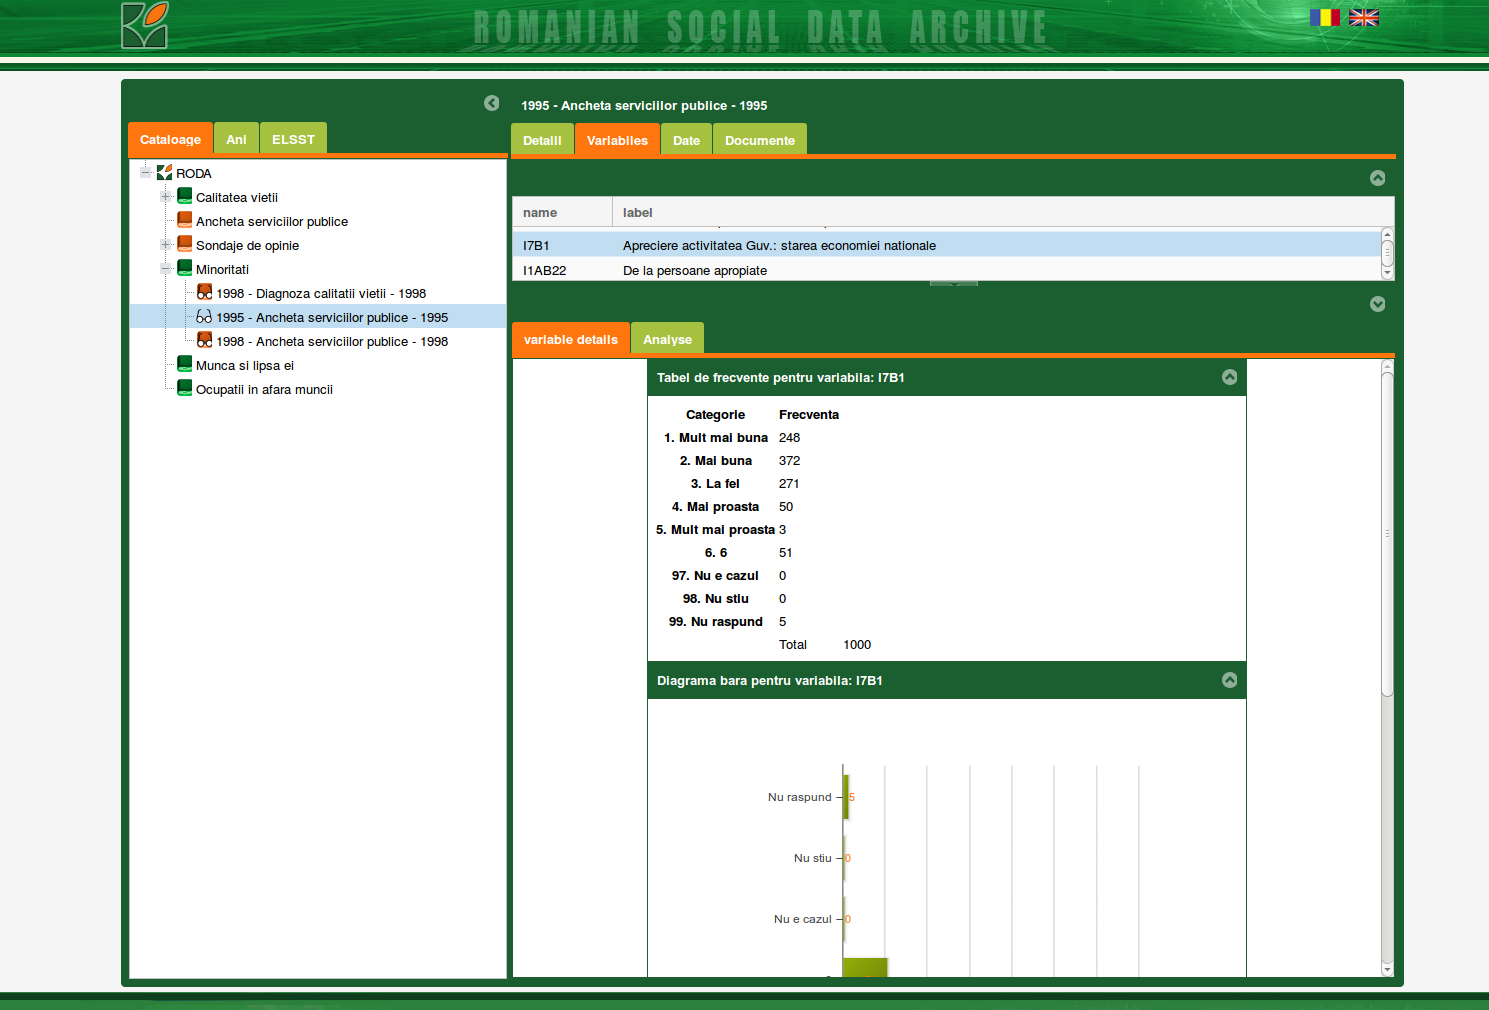
\includegraphics[width=16cm]{img/Screenshot-statistics}

Contructia tabelelor si graficelor se face pe baza raspunsului venit de la server in format JSON care arata dupa cum urmeaza:


\begin{lstlisting}[language=json]

{
    "success": true,
    "data": [
        {
            "itemtype": "table",
            "title": "Masuri numerice pentru variabilele: v1 si v2",
            "headerRow": 1,
            "headerCol": 1,
            "rows": 7,
            "cols": 3,
            "data": [
                ["", "v1", "v2"],
                ["Min.", "1", "19"],
                ["1st Qu.", "4", "36"],
                ["Median", "6", "53"],
                ["Mean", "5.6", "54"],
                ["3rd Qu.", "8", "71"],
                ["Max.", "10", "90"]
            ]
        },{
            "itemtype": "table",
            "title": "Corelatia dintre variabilele: v1 si v2",
            "headerRow": 1,
            "headerCol": 1,
            "rows": 2,
            "cols": 2,
            "data": [
                ["", "v2"],
                ["v1", "0.144"]
            ]
        },{
            "itemtype": "chart",
            "title": "Diagrama de imprastiere pentru variabilele: v1 si v2",
            "charttype": "scatterplot",
            "height": 500,
            "data": [...]
            ]
        }
    ]
}
\end{lstlisting}

In cazul in care analiza este facuta pe doua variabile, rezultatul arata ca in figura urmatoare:

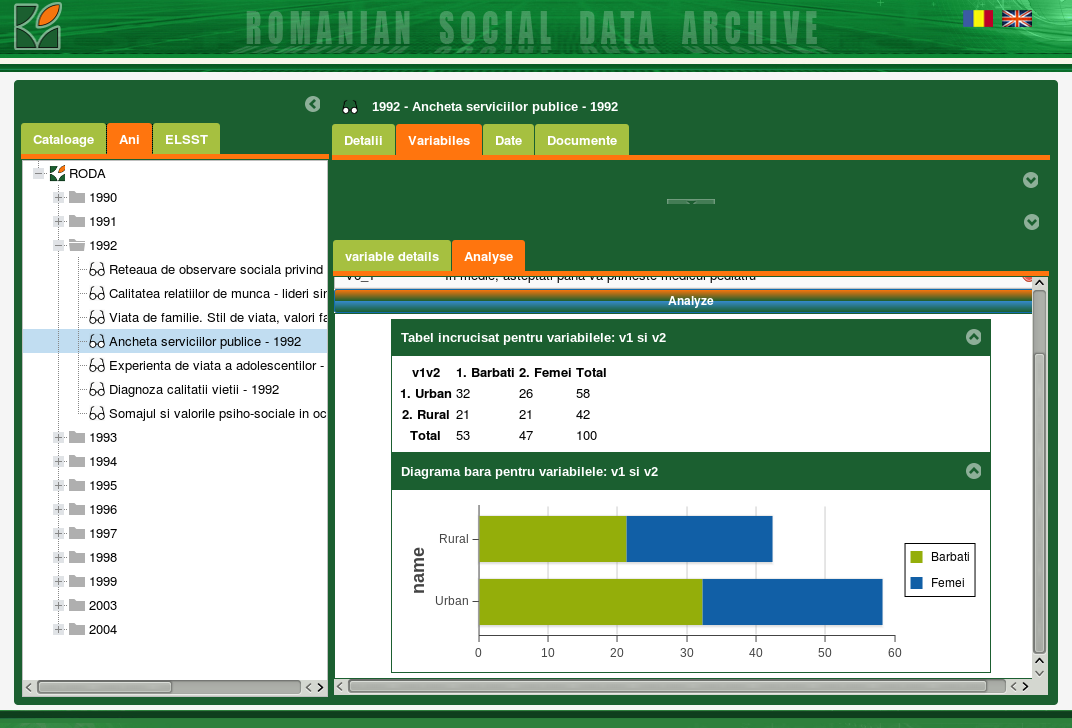
\includegraphics[width=16cm]{img/db-bivar}


iar datele care vin de la motorul statistic arata dupa cum urmeaza:

\begin{lstlisting}[language=json]

{
    "success": true,
    "data": [
        {
            "itemtype": "table",
            "title": "Tabel incrucisat pentru variabilele: v1 si v2",
            "headerRow": 1,
            "headerCol": 1,
            "rows": 4,
            "cols": 4,
            "data": [
                ["v1v2", "1. Barbati", "2. Femei", "Total"],
                ["1. Urban", "32", "26", "58"],
                ["2. Rural", "21", "21", "42"],
                ["Total", "53", "47", "100"]
            ]
        },{
            "itemtype": "chart",
            "title": "Diagrama bara pentru variabilele: v1 si v2",
            "charttype": "stackedbar",
            "catfield": "name",
            "datafield1": "Barbati",
            "datafield2": "Femei",
            "height": 170,
            "data": [
                {
                    "name": "Urban",
                    "Barbati": 32,
                    "Femei": 26
                },
                {
                    "name": "Rural",
                    "Barbati": 21,
                    "Femei": 21
                }
            ]
        }
    ]
}

\end{lstlisting}

\section{Constructia raspunsului grafic la datele statistice}

Toate modulele de admistrare sau de acces la date care sunt construite cu ajutorul bibliotecilor ExtJS au in comun un detaliu de arhitectura: Se stie exact ce trebuie sa se afiseze in fiecare stare a intrfetei, oricat ar fi aceasta de complexa. In cazul raspunsului la datele statistice situatia este diferita, componentul de afisare a acestuia trebuie construit dupa aparitia raspunsului de la server. Pentru aceasta a trebuit construit un sistem aparte compus dintr-un controller special si o serie de componente predefinite care sa se poata utiliza pentru constructia graficelor, obtinute prin extinderea componentelor disponibile in continutul bibliotecii extjs

Graficele predefinite sunt urmatoarele: 

\begin{itemize}
\item 'databrowser.view.StackedBarChart'
\item 'databrowser.view.FrequencyChart'
\item 'databrowser.view.ScatterChart'
\item 'databrowser.view.PieChart'
\end{itemize}


Componentele obtinute prin extinderea graficelor sunt construite in asa fel incat sa poata obtine numele seriilor de date in momentul constructiei, spre deosebire de componentele pentru grafice ale ExtJS-ului care solicita specificarea acestora in momentul constructiei. 

Prelucrarea jsonului de raspuns se face de catre controllerul numit 'databrowser.controller.DataBrowser'. In momentul in care datele sosesc de la motorul statistic, controllerul se asteapta sa gaseasca in raspunsul JSON unul dintre urmatoarele tipuri de obiecte:

\begin{itemize}

\item paragraf. Paragraful este un text cu titlu care se afiseaza intr-un panou separat. Este conceput fie pentru mesaje de eroare fie pentru texte care trebuiesc afisate in functie de rezultatul analizei. Structura de date a unui paragraf este urmatoarea: 

\begin{lstlisting}[language=json]
		{
            "itemtype": "paragraph",
            "title": "Titlul paragrafului",
            "contenrt": "Continutul paragrafului",
        },
\end{lstlisting}

\item Tabel Tabelul este folosit pentru afisarea datelor tabelare care pot proveni din mai multe surse. In cazul analizelor variabilelor numerice se pot afisa parametrii statistici de baza (medie, percentile) intr-un fomrat tabelar. Formatul asteptat pentru un tabel este urmatorul: 

\begin{lstlisting}[language=json]
       {
            "itemtype": "table",
            "title": "Titlul tabelului",
            "headerRow": 1,
            "headerCol": 1,
            "rows": 4,
            "cols": 4,
            "data": [
                ["v1/v2", "1. Barbati", "2. Femei", "Total"],
                ["1. Urban", "32", "26", "58"],
                ["2. Rural", "21", "21", "42"],
                ["Total", "53", "47", "100"]
            ]
        }
\end{lstlisting}

JSON-ul trebuie sa specifice daca tabelul are header (titluri ale coloanelor sau randurilor), numarul total de randuri si numarul total de coloane. 


\item chart Sectiunea in care se specifica datele si proprietatile unui grafic. Formatele difera putin in functie de tipul de grafic dar toate au in comun specificarea tipului de grafic, numele seriilor, titlul graficului si sectiunea de date. 


\end{itemize}

Procedeul de constructie implica impartirea raspunsului pe sectiuni principale. Pentru fiecare sectiune principala, in functie de tipul acesteia se adauga un component de tip 'Ext.panel.Panel' la panoul care contine rapsunsul iar in acest component, in functie de tipul de component, fie se instantiaza un component nou de tip chart, fie se introduce un component de tip 'Ext.XTemplate' care pe baza continutului jsonului construieste fie tabelul fie paragraful. 




